\section{Evaluation}
\label{sec:evaluation}

The final evaluation is populated by the claim-audited output of
\texttt{python -m bench.analyze\_final}. The script refuses to run until all
48 declared conditions are terminal and keeps any harness-invalid condition in
explicit exclusion accounting. This section is organized by research question
rather than by implementation component.

\subsection{RQ1: What does the pass-through layer cost?}

\ProxyFinding

\IfFileExists{figures/primary_overview.pdf}{
\begin{figure*}[t]
  \centering
  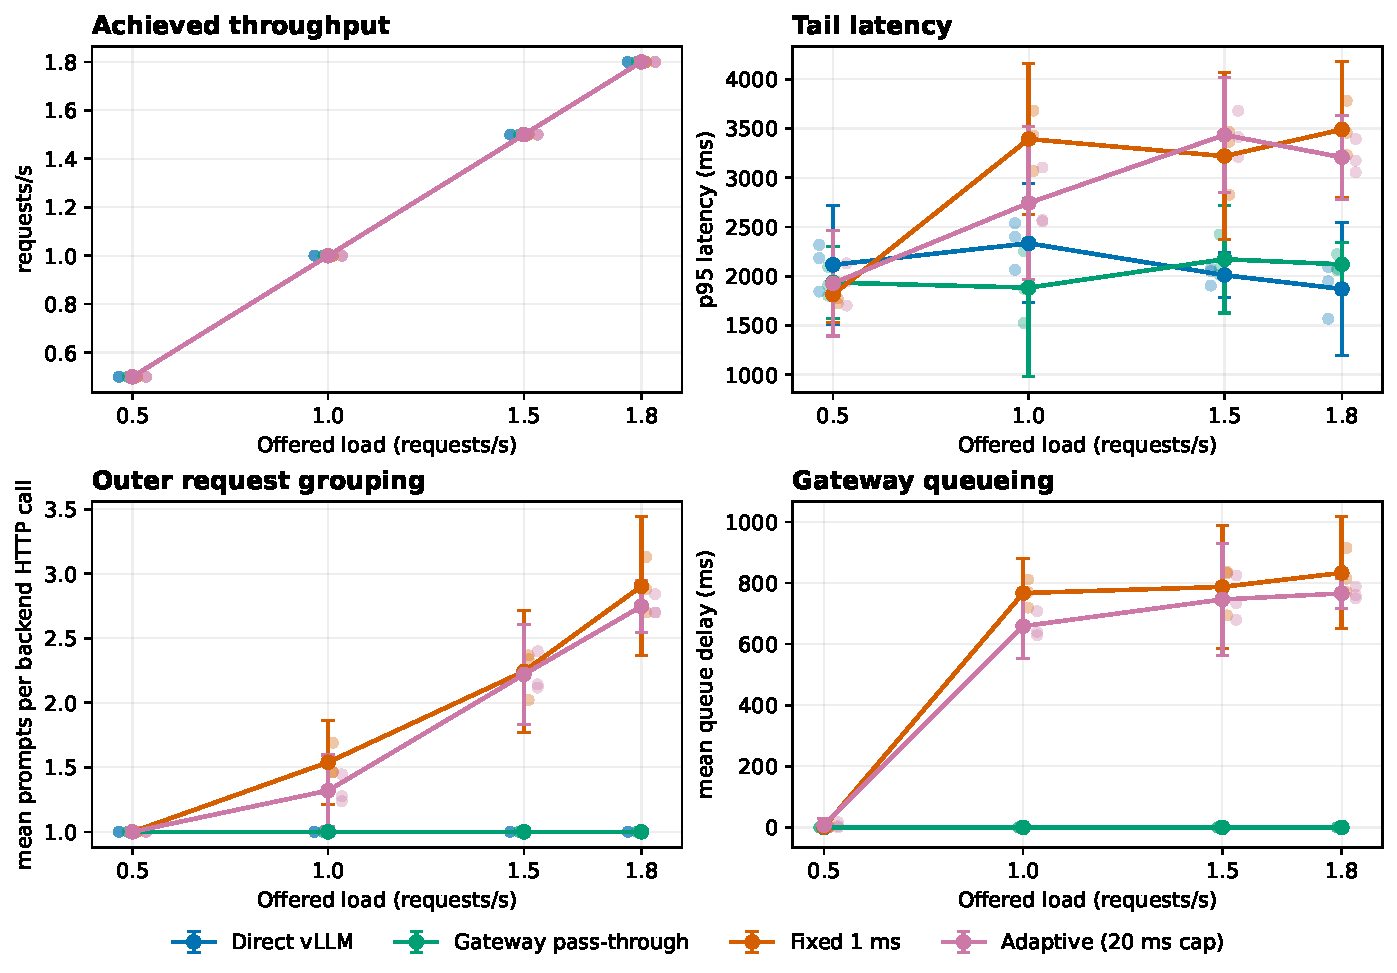
\includegraphics[width=0.96\textwidth]{figures/primary_overview.pdf}
  \caption{Primary matrix on \model{} and one \gpu{}. Lines show means across
  three run-level repetitions; error bars are two-sided 95\% Student-$t$
  intervals; translucent points are individual repetitions. Offered load is
  fixed by the open-loop schedule. Outer request grouping is call-weighted
  prompts per backend HTTP call, not \vllm{}'s token-level active set.}
  \label{fig:overview}
\end{figure*}
}{}

\subsection{RQ2: Does fixed outer batching help?}

\PrimaryFinding

\IfFileExists{tables/primary_results.tex}{
\begin{table*}[t]
  \centering
  \small
  \caption{All primary conditions. Values are run-level mean $\pm$ 95\%
  Student-$t$ half-width over three repetitions. Throughput is achieved
  successful requests/s.}
  \label{tab:primary}
  \resizebox{\textwidth}{!}{% Generated by python -m bench.analyze_final; do not edit by hand.
\begin{tabular}{llrrrr}
\toprule
Mode & Rate & Throughput & p95 latency & Outer group & Queue delay \\
 & (req/s) & (req/s) & (ms) & (requests) & (ms) \\
\midrule
Direct vLLM & 0.5 & 0.50 $\pm$ 0.00 & 2115 $\pm$ 607 & 1.00 $\pm$ 0.00 & -- \\
Direct vLLM & 1.0 & 1.00 $\pm$ 0.00 & 2334 $\pm$ 605 & 1.00 $\pm$ 0.00 & -- \\
Direct vLLM & 1.5 & 1.50 $\pm$ 0.00 & 2010 $\pm$ 229 & 1.00 $\pm$ 0.00 & -- \\
Direct vLLM & 1.8 & 1.80 $\pm$ 0.00 & 1870 $\pm$ 674 & 1.00 $\pm$ 0.00 & -- \\
\addlinespace
Gateway pass-through & 0.5 & 0.50 $\pm$ 0.00 & 1935 $\pm$ 367 & 1.00 $\pm$ 0.00 & 0 $\pm$ 0 \\
Gateway pass-through & 1.0 & 1.00 $\pm$ 0.00 & 1884 $\pm$ 906 & 1.00 $\pm$ 0.00 & 0 $\pm$ 0 \\
Gateway pass-through & 1.5 & 1.50 $\pm$ 0.00 & 2172 $\pm$ 546 & 1.00 $\pm$ 0.00 & 0 $\pm$ 0 \\
Gateway pass-through & 1.8 & 1.80 $\pm$ 0.00 & 2120 $\pm$ 223 & 1.00 $\pm$ 0.00 & 0 $\pm$ 0 \\
\addlinespace
Fixed 1 ms & 0.5 & 0.50 $\pm$ 0.00 & 1812 $\pm$ 280 & 1.00 $\pm$ 0.00 & 2 $\pm$ 1 \\
Fixed 1 ms & 1.0 & 1.00 $\pm$ 0.00 & 3393 $\pm$ 763 & 1.54 $\pm$ 0.33 & 767 $\pm$ 114 \\
Fixed 1 ms & 1.5 & 1.50 $\pm$ 0.00 & 3220 $\pm$ 850 & 2.24 $\pm$ 0.48 & 788 $\pm$ 201 \\
Fixed 1 ms & 1.8 & 1.80 $\pm$ 0.00 & 3490 $\pm$ 687 & 2.90 $\pm$ 0.54 & 833 $\pm$ 183 \\
\addlinespace
Adaptive (20 ms cap) & 0.5 & 0.50 $\pm$ 0.00 & 1927 $\pm$ 535 & 1.00 $\pm$ 0.00 & 7 $\pm$ 21 \\
Adaptive (20 ms cap) & 1.0 & 1.00 $\pm$ 0.00 & 2744 $\pm$ 777 & 1.32 $\pm$ 0.28 & 659 $\pm$ 106 \\
Adaptive (20 ms cap) & 1.5 & 1.50 $\pm$ 0.00 & 3435 $\pm$ 583 & 2.22 $\pm$ 0.39 & 746 $\pm$ 182 \\
Adaptive (20 ms cap) & 1.8 & 1.80 $\pm$ 0.00 & 3208 $\pm$ 426 & 2.75 $\pm$ 0.20 & 766 $\pm$ 50 \\
\bottomrule
\end{tabular}
}
\end{table*}
}{}

\IfFileExists{figures/mechanism_effects.pdf}{
\begin{figure*}[t]
  \centering
  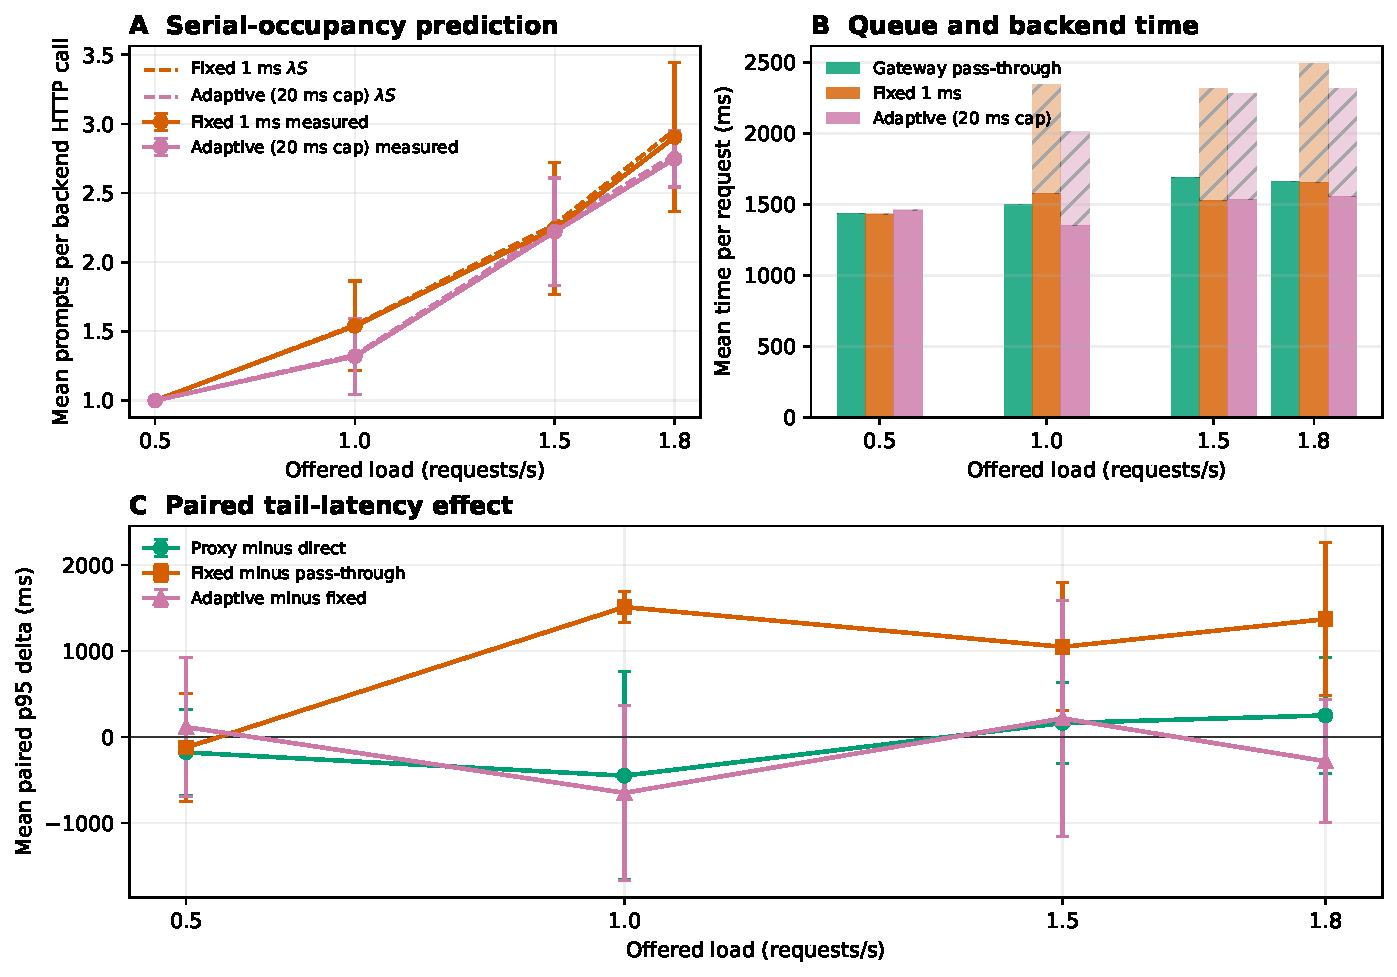
\includegraphics[width=0.96\textwidth]{figures/mechanism_effects.pdf}
  \caption{Mechanism accounting for \model{} on one \gpu{}. Panel A compares
  measured call-weighted outer grouping with the serial-occupancy prediction
  $\max(1,\lambda\bar S_{\mathrm{call}})$. Panel B separates gateway queue
  and backend time; hatching denotes queue time stacked above backend time.
  Panel C shows paired p95-latency effects by repetition seed. Error bars are
  two-sided 95\% Student-$t$ intervals over three run-level values or paired
  differences.}
  \label{fig:mechanism}
\end{figure*}
}{}

\subsection{RQ3: Does the frozen adaptive policy help?}

\AdaptiveFinding

\IfFileExists{tables/paired_effects.tex}{
\begin{table}[t]
  \centering
  \scriptsize
  \caption{Paired p95-latency effects. Positive values mean the treatment is
  slower than its comparator. Values are mean $\pm$ 95\% Student-$t$
  half-width across shared repetition seeds.}
  \label{tab:effects}
  \resizebox{\columnwidth}{!}{% Generated by python -m bench.analyze_final; do not edit by hand.
\begin{tabular}{lrrr}
\toprule
Comparison & Rate & p95 delta (ms) & Relative delta (\%) \\
\midrule
Proxy minus direct & 0.5 & -180 $\pm$ 496 & -8.0 $\pm$ 20.9 \\
Proxy minus direct & 1.0 & -451 $\pm$ 1212 & -18.4 $\pm$ 46.4 \\
Proxy minus direct & 1.5 & 162 $\pm$ 472 & 8.0 $\pm$ 22.9 \\
Proxy minus direct & 1.8 & 251 $\pm$ 675 & 15.0 $\pm$ 42.3 \\
Fixed minus pass-through & 0.5 & -123 $\pm$ 631 & -5.7 $\pm$ 31.6 \\
Fixed minus pass-through & 1.0 & 1510 $\pm$ 180 & 82.6 $\pm$ 47.3 \\
Fixed minus pass-through & 1.5 & 1047 $\pm$ 744 & 48.7 $\pm$ 40.2 \\
Fixed minus pass-through & 1.8 & 1370 $\pm$ 886 & 65.1 $\pm$ 47.6 \\
Adaptive minus fixed & 0.5 & 115 $\pm$ 811 & 7.1 $\pm$ 45.0 \\
Adaptive minus fixed & 1.0 & -650 $\pm$ 1019 & -18.8 $\pm$ 26.1 \\
Adaptive minus fixed & 1.5 & 216 $\pm$ 1373 & 8.0 $\pm$ 47.6 \\
Adaptive minus fixed & 1.8 & -282 $\pm$ 713 & -7.8 $\pm$ 18.4 \\
\bottomrule
\end{tabular}
}
\end{table}
}{}

\subsection{Validity and negative-result accounting}

The final paper reports the exact number of complete, harness-invalid, failed,
and interrupted runs. Interrupted attempts are operational history, not
samples. Any harness-invalid terminal condition remains visible with its
predeclared reason but contributes to no performance mean. If fewer than three
valid repetitions remain for a condition, we report the reduced $n$ and avoid
a confirmatory claim for that comparison.
